\chapter{Modulating Sound}

One of the most interesting aspects of any synthesizer, digital as well as analog, is its capability to modify or \emph{modulate} sound in a variety of ways. To modulate a sound means to change its amplitude, pitch, timbre, or any other property of a signal to produce an, often entirely, new sound. This chapter will examine and explain two of the most popular means of modulation in a digital synthesis system, Envelopes and Low Frequency Oscillators (LFOs).

\section{Envelopes}

When a pianist hits a key on a piano, the amplitude of the sound produced increases from zero, no sound, to some maximum amplitude which depends on a multitude of factors such as how hard the musician pressed the key, what material the piano string is made of, the influence of air friction and so on. After reaching the maximum loudness, the amplitude decreases until the piano string stops oscillating, resulting in renewed silence. To model such an evolution of amplitude over time, digital musicians use a modulation technique commonly referred to as an "Envelope".

\subsection{Envelope segments}

The following sections outline the creation of and terminology used for single segments of an envelope.

\subsubsection{ADSR}

A common concept associated with Envelopes is "ADSR", which stands for "Attack, Decay, Sustain, Release". These four terms name the four possible states an Envelope segment can take on. An Attack segment is any segment where the initial amplitude, at the start of a segment, is less than the final amplitude, at the end of the segment --- the amplitude increases. Conversely, a Decay segment signifies a decrease in amplitude from a higher to a lower value. When the loudness of a signal stays constant for the full duration of an interval, this interval is termed a "Sustain" segment. While the three segment types just mentioned all describe the modulation of a signal's loudness when the key of a piano or synthesizer is still being pressed, the last segment type, a "Release" segment, refers to the change in loudness once the key is \emph{released}. Figure \ref{fig:adsr} depicts an abstract representation of a typical ADSR envelope. Figure \ref{fig:envb} shows a 440 Hz sine wave before the application of an ADSR envelope and Figure \ref{fig:enva} displays the same signal after an ADSR envelope has been applied to it.

\begin{figure}[p!]
  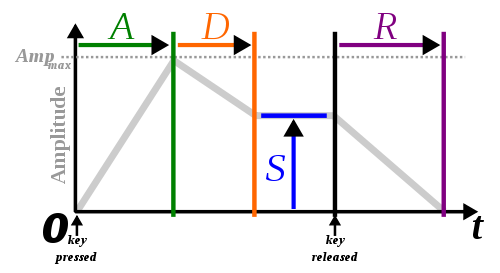
\includegraphics[scale=0.8]{img/adsr}
  \caption{An Envelope with an Attack, a Decay, a Sustain and finally a Release segment. Source: \protect\url{http://upload.wikimedia.org/wikipedia/commons/thumb/e/ea/ADSR_parameter.svg/500px-ADSR_parameter.svg.png}}
  \label{fig:adsr}
\end{figure}

\begin{figure}[p!]
  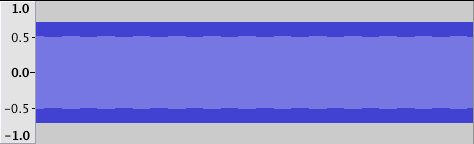
\includegraphics[scale=0.8]{img/envb}
  \caption{A 440 Hz sine wave.}
  \label{fig:envb}
\end{figure}

\begin{figure}[p!]
  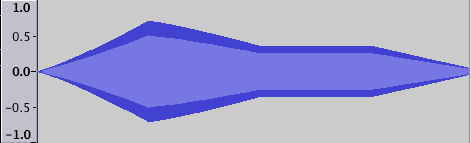
\includegraphics[scale=0.8]{img/enva}
  \caption{The same signal from Figure \ref{fig:envb} with an ADSR Envelope overlayed on it.}
  \label{fig:enva}
\end{figure}

\subsubsection{Mathematical Definition and Rate Types}

Mathematically, an Envelope segment can be modeled using a simple power function of the general form presented in Equation \ref{eq:power}, where $a_{final}$ is the final amplitude at the end of the segment, $a_{start}$ the initial amplitude at the beginning of the segment and $r$ the parameter responsible for the shape or "rate" of the segment. When $r$, which must kept between $0$ and $\infty$ (practically speaking some value around $10$), is equal to $1$, the segment has a linear rate and is thus a straight line connecting the initial amplitude with the final loudness. If $r$ is greater than 1, the function becomes a power function and consequently exhibits a non-linear increase or decrease in amplitude. Lastly, if $r$ is less than 1 but greater than 0, the function is termed a "radical function", since any term of the form $x^\frac{a}{b}$ can be re-written to the form $\sqrt[b]{x^a}$, where the numerator $a$ becomes the power of the variable and the denominator $b$ the radicand. Figure \ref{fig:rates} displays an envelope whose first segment has $r = 2$, a quadratic increase, after which the sound decays linearly, before increasing again, this time $r$ being equal to $\frac{1}{2}$ (a square root function). A C++ class for single Envelope segments is shown in Listing \ref{code:envseg}.

\begin{equation}
  a(t) = (a_{final} - a_{start}) \cdot t^r + a_{start}
  \label{eq:power}
\end{equation}

\begin{figure}
  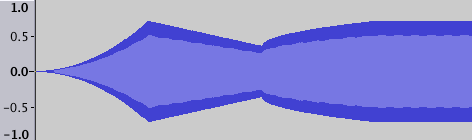
\includegraphics[scale=0.7]{img/rates}
  \caption{An envelope where $r$ is equal to 2, then to 1, then to 0.5.}
  \label{fig:rates}
\end{figure}

\subsection{Full Envelopes}

Creating full Envelopes with a variable number of segments requires little more work than implementing a state-machine, which checks whether the current sample count is greater than the length of the Envelope segment currently active. If the sample count is still less than the length of the segment, one retrieves Envelope values from the current segment, else the Envelope progresses to the next segment. Additionally, it should be possible for the user to loop between segments of an Envelope a variable number of times before moving on to the release segment. Table \ref{code:envsegseq} displays two member functions of an Envelope class created for this thesis, which return an Envelope value from the current Envelope segment and allow for the updating of the sample count.

\begin{table}
  \code{envsegseq.cpp}
  \caption{Two member functions of the EnvSegSeq class (Envelope Segment Sequence).}
  \label{code:envsegseq}
\end{table}

\noindent Envelopes have many uses. Some require flexible segments which allow for the adjusting of individual segments' lengths, others need all segments to have a constant length. Some give the user the possibility to modulate individual segments by making them behave like a sine function, others do not. Fortunately, C++'s inheritance features make it very easy and efficient to construct such a variety of different classes that may or may not share relevant features. The inheritance diagram for the final \texttt{Envelope} class created for the purpose of this thesis reflects how all of these individual class can play together to yield the wanted features for a class. This inheritance diagram is displayed in Figure \ref{fig:envelope-inherit}.

\begin{figure}
  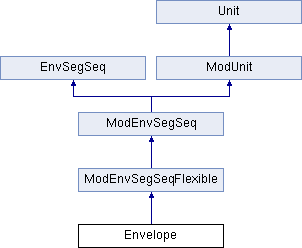
\includegraphics[scale=0.7]{img/envelope-inherit}
  \caption{The inheritance diagram for the \texttt{Envelope} class. The \texttt{Unit} and \texttt{ModUnit} classes are two abstract classes that will be explained in later parts of this thesis.}
  \label{fig:envelope-inherit}
\end{figure}

\section{Low Frequency Oscillators}

A Low Frequency Oscillator, abbreviated "LFO", is an oscillator operating at very low frequencies, typically in the range below human hearing (0-20 Hz), used solely for the purposes of modulating other signals. The most common parameter to be modulated by an LFO in a synthesizer is the amplitude of another oscillator, to produce effects such as the well known "vibrato" effect. In this case, were the frequency of the LFO to be in the audible range, one would use the term Amplitude Modulation (AM), which is also a method for synthesizing sound. Equation \ref{eq:lfoam} shows how an LFO can be used to change the amplitude of another oscillator\footnote{This is the same equation as for AM.}. Figure \ref{fig:lfo1} shows a 440 Hz sine wave, Figure \ref{fig:lfo2} displays the same sine wave now modulated by a 2 Hz LFO and in Figure \ref{fig:lfo3} the frequency of the LFO has been increased to 20 Hz to produce a vibrato effect. It should be noted that an LFO can also modulate any other parameter, such as the rate of an Envelope segment.

\begin{equation}
  O(t) = (A_{osc} + (A_{lfo} \cdot sin(\omega_{lfo}t + \phi_{lfo}))) \cdot sin(\omega_{osc}t + \phi_{osc})
  \label{eq:lfoam}
\end{equation}

\begin{figure}[h!]
  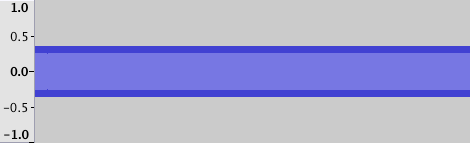
\includegraphics[scale=0.5]{img/lfo1}
  \caption{A 440 Hz sine wave.}
  \label{fig:lfo1}
\end{figure}

\begin{figure}[h!]
  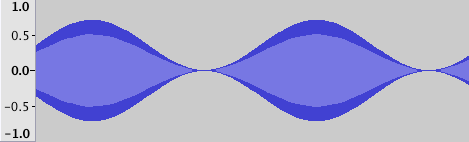
\includegraphics[scale=0.5]{img/lfo2}
  \caption{The sine wave from Figure \ref{fig:lfo1} modulated by an LFO with a frequency of 2 Hertz. Note how the maximum amplitude of the underlying signal now follows the waveform of a sine wave. Because the LFO's amplitude is the same as that of the oscillator (the "carrier" wave), the loudness is twice as high at its maximum, and zero at its minimum.}
  \label{fig:lfo2}
\end{figure}

\begin{figure}[h!]
  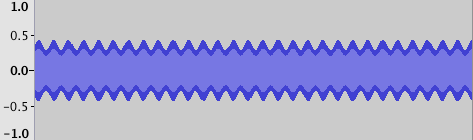
\includegraphics[scale=0.5]{img/lfo3}
  \caption{The sine wave from Figure \ref{fig:lfo1} modulated by an LFO with a frequency of 20 Hertz. This signal is said to have a "vibrato" sound to it.}
  \label{fig:lfo3}
\end{figure}

\pagebreak

\noindent Concerning the implementation of an LFO in a computer program, the process could be as simple as re-naming a class used for an oscillator:

\begin{lstlisting}
  typedef OscillatorClass LFOClass.
\end{lstlisting}

\noindent In the synthesizer created for this thesis, called \emph{Anthem}, the distinction between an LFO and an oscillator is the possibility to modulate an LFO's parameters, for example using an Envelope or another LFO, whereas the \texttt{Oscillator} class is an abstract base class whose sole purpose is to be an interface to a Wavetable. This property of the \texttt{Oscillator} class is used by both the \texttt{LFO} and the \texttt{Operator} class, who both inherit from the \texttt{Oscillator} class. The \texttt{Operator} class is the sound generation unit the user actually interfaces with from the Graphical User Interface (GUI) of \emph{Anthem}. It is derived from the \texttt{Oscillator} class because it ultimately needs to generate sound samples, but it is its own class because it has various other features used for sound synthesis. These features are discussed in a later chapter. The relationships just described lead to the inheritance diagram shown in Figure \ref{fig:osc-derived}.

\begin{figure}[h!]
  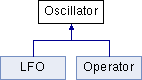
\includegraphics[scale=0.9]{img/osc-derived}
  \caption{Inheritance diagram showing the relationship between an \texttt{LFO}, an \texttt{Operator} and their base class, the \texttt{Oscillator} class.}
  \label{fig:osc-derived}
\end{figure}

\subsection{LFO Sequences}

A common sight in many modern digital synthesizers, such as Native Instruments'\footnotemark{} "Massive" synthesizer, is a form of step-sequencer for Low Frequency Oscillators. This modulation unit is essentially a synthesis between the concept of an Envelope and that of an LFO. It has a variable number of segments of fixed length, each with their own LFO to change the waveform of the segment. Figure \ref{fig:lfoseq} displays what Native Instruments calls a "Stepper".

\footnotetext{"Native Instruments is a technology company that develops software and hardware for music production and DJ-ing", based out of Berlin, Germany. Source: \emph{Wikpedia:} \url{http://en.wikipedia.org/wiki/Native_Instruments}. Homepage: \url{http://www.native-instruments.com/en/}}

\begin{figure}
  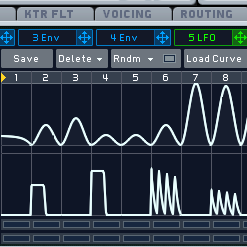
\includegraphics[scale=0.6]{img/lfoseq}
  \caption{An LFO sequence, here named a "Stepper". Source: \protect\url{http://www.askaudiomag.com/articles/massives-performer-and-stepper-lfos}}
  \label{fig:lfoseq}
\end{figure}

For the purpose of this thesis, such an LFO sequence was created. Regarding the implementation in C++, there is little difference between an LFO Sequence and an Envelope Segment Sequence, except for the fact that now each individual segment has an LFO that can be accessed through the interface of the class to change the parameters or the waveform of each LFO. One of the two parameters that deserves to be discussed, however, is the frequency or "rate" of such an LFO sequence. Just like the frequency of an oscillator describes the number of cycles its waveform completes every second, the rate of an LFO Sequence determines how often the entire sequence is traversed in one second. Practically speaking, this involves adjusting the length of individual segments in such a way that the combined length equals the wanted duration. To give an example: if the user wishes to change the rate of an LFO Sequence with 10 segments to 1 Hz, each individual segment must have a duration of 0.1 seconds (100 milliseconds), so that at the end of the sequence, exactly $10 \text{ segments} \cdot 0.1 \text{ seconds} = 1 \text{ second}$ will have passed. The length of a single segment can be derived from Equation \ref{eq:lfoseq1}, where $r$ is the rate of the LFO Sequence and $N$ the number of segments in the sequence.

\begin{equation}
  l_{seg} = \frac{1}{r \cdot N}
  \label{eq:lfoseq1}
\end{equation}

\noindent The second parameter worthy of mentioning is the frequency of individual segments' modulation LFOs. As mentioned, the frequency of an oscillator or of an LFO sets the cycles per second of their waveform. However, when the length of a single segment in an LFO sequence is only very small, e.g. 100 milliseconds, having an LFO modulate the segment at a common frequency of, say, 1 Hz, would mean that only one tenth of the LFO's period is completed. To have the LFO complete a full cycle, the user would have to adjust the frequency of the LFO in such a way that it can complete one period within the duration of the segment (in this case, 10 Hz). This may still seem like a manageable task for the user. However, once parameter values become a little more complicated, giving birth to cases where the user has to figure out that to have 5 cycles in a segment with a duration of 0.4 seconds, the frequency needs to be exactly 12.5 Hz, the objective reader must admit that this is not intuitive behaviour. Therefore, it was decided that for modulation LFOs in LFO sequences, the rate should not be defined as cycles per second, but as cycles per \emph{segment}. This means that setting the rate of a segment's LFO to 5 Hertz results in 5 cycles per second regardless of the segment's duration. Naturally, the task of calculating the correct frequency for the LFO still has to be performed by the computer program. The real frequency can be calculated using Equation \ref{eq:lfoseq2} when the duration $d$ is in seconds and Equation \ref{eq:lfoseq3} when the duration is in samples, as is the case for a digital synthesizer. In both Equations $f_{displayed}$ stands for the frequency the user specifies, the cycles per segment, and $f_{real}$ for the actual frequency in cycles per second. In Equation \ref{eq:lfoseq3}, $f_{s}$ denotes the sample rate. Table \ref{code:lfoseq} shows how the calculation of the two parameters just dicussed is implemented in the \texttt{LFOSeq} class.

\begin{equation}
  f_{real} = \frac{f_{displayed}}{d}
  \label{eq:lfoseq2}
\end{equation}

\begin{equation}
  f_{real} = \frac{f_{s}}{d} \cdot f_{displayed}
  \label{eq:lfoseq3}
\end{equation}

\begin{table}[p!]
  \code{lfoseq.cpp}
  \caption{Relevant member functions from the \texttt{LFOSeq} class for calculating the correct rate for individual segments as well as for the entire sequence.}
  \label{code:lfoseq}
\end{table}

\pagebreak

\section{The ModDock system}

The majority of digital synthesizers, such as Propellerhead's\footnotemark{} \emph{Thor} or Native Instruments'\footnotemark[2] \emph{FM8} synthesizer, implement modulation in a static way. Instead of making it possible to use an LFO or an Envelope to modulate any parameter in a synthesis system, units, e.g. an oscillator, have dedicated LFOs and Envelopes, which modulate only one parameter --- mostly amplitude --- and only for this unit. On the other hand, some synthesizers like \emph{Massive}, also created by Native Instruments, implement a system where LFOs and Envelopes can be used by a variable number of units, for a variable number of parameters. For this thesis and the synthesizer created for it, such a system, here called the "ModDock" system, was emulated. The following sections will outline the process of defining and implementing the ModDock system.

\footnotetext{"Propellerhead Software is a music software company, based in Stockholm, Sweden, and founded in 1994." Source: \emph{Wikipedia} \url{http://en.wikipedia.org/wiki/Propellerhead_Software}. Homepage: \url{https://www.propellerheads.se}}

\subsection{Problem statement}

In short, the ModDock system should make it possible to modulate a variable number of parameters of a variable number of units of the synthesizer, with any of a fixed number of LFOs, Envelopes or similar \emph{Modulation Units}. Consequently, each unit in the synthesis system should have what will be known as a "ModDock", a set of "docks", the number of which depends on the number of parameters the unit makes it possible to modulate, where the user may insert a Modulation Unit. Due to the fact that many units may be modulated by one Modulation Unit, the Modulation Unit must not update its value until all units have been modulated by it. For example, the sample count of an Envelope must stay the same until all dependent units have retrieved the current Envelope value from it. Moreover, a unit should be able to adjust the depth of modulation by a Modulation Unit, i.e. it should be possible to have only 50\% of an LFO's signal affect the parameter it is modulating. Finally, there should be a way of \emph{side-chaining} Modulation Units so that one Modulation Unit in a dock modulates the depth of another Modulation Unit in that same dock, the signal of which may again side-chain the depth of another Modulation Unit in that ModDock. The final modulation of a parameter will be the average of all modulation values of a ModDock affecting that parameter.

\subsection{Implementation}

In order to let units of the synthesizer created for this thesis share certain behaviour and member functions, as well as to distinguish between the traits and tasks certain units have that others do not, it was necessary to develop an inheritance structure that would satisfy these requirements. In \emph{Anthem}, a \emph{Unit} is defined as any object with modulateable parameters. A Unit has necessary member variables and functions to permit its parameters to be modulated by other \emph{Modulation Units}. A Modulation Unit, short \emph{ModUnit}, shall be defined as any Unit that can modulate a parameter of a Unit. The ModUnit class includes the \emph{pure virtual}\footnotemark{} \texttt{modulate} method, which takes a sample as one of its arguments and then returns a modulated version of that sample. The form of modulation depends entirely on the implementation of the \texttt{modulate} method by the class that inherits from the ModUnit class, as the ModUnit class itself does not implement any standard way of modulating a sample. Figure \ref{fig:unit-inherit} displays the inheritance diagram for the Unit class.

\begin{figure}
  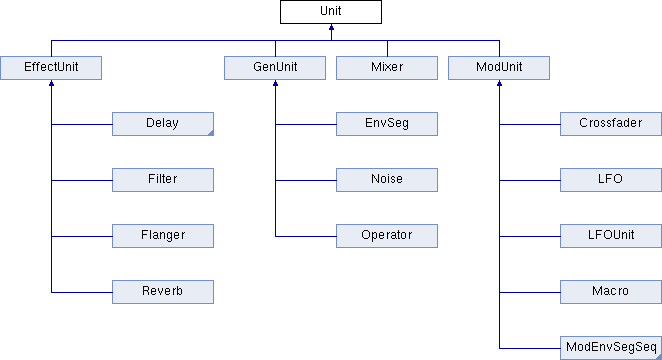
\includegraphics[scale=0.5]{img/unit-inherit}
  \caption{The inheritance diagram of the Unit class. GenUnits are Units that generate samples. EffectUnits apply some effect to a sample, e.g. a sample delay.}
  \label{fig:unit-inherit}
\end{figure}

\footnotetext{In C++, a pure virtual function is a function that does not have any standard implementation and thus requires the derived classes of the class that declares the pure virtual function to implement that function on their own. A class that declares a pure virtual method is termed an \emph{abstract} class and may not be instantiated.}

\subsubsection{The \texttt{modulate} method}

All classes derived from the ModUnit class must implement the \texttt{modulate} method, which takes the sample to modulate, a depth value between 0 (no modulation) and 1 (full modulation) as well as a maximum boundary as its arguments. In the case of LFOs, the maximum boundary parameter determines the value that is added to the sample. For example, when the amplitude of a unit is modulated, the maximum boundary is 1, meaning that the value added to the sample is in the range of $[-A_{LFO} \cdot 1; A_{LFO} \cdot 1]$, whereas for the rate parameter of Envelope segments, where the maximum boundary is 10, the range is $[-A_{LFO} \cdot 10; A_{LFO} \cdot 10]$. The declaration of the \texttt{modulate} method in the ModUnit class is given below.

\begin{lstlisting}
  virtual double modulate(double sample, double depth, double maximum) = 0;
\end{lstlisting}

This method was the main motivation behind the creation of the ModUnit class and is especially important for ModDocks, as it makes it possible to polymorphically access the \texttt{modulate} method of any ModUnit through a pointer-to-ModUnit (\texttt{ModUnit*}). This means that each ModUnit can have its own definition of what it means to modulate a sample. Table \ref{code:modlfo} shows the definition of the \texttt{modulate} method in the LFO and Table \ref{code:modenv} in the Envelope class.

\begin{table}[h!]
  \code{modlfo.cpp}
  \caption{The implementation of the \texttt{modulate} method for LFOs.}
  \label{code:modlfo}
\end{table}

\begin{table}[h!]
  \code{modenv.cpp}
  \caption{The implementation of the \texttt{modulate} method for Envelopes. Note that for the Envelope class, the paramter \texttt{maximum} is not relevant, which is why it is never used. This shows that all that matters is that the method returns a modulated sample --- what "modulate" means is up to the class that implements it.}
  \label{code:modenv}
\end{table}

\pagebreak

\subsubsection{ModDocks}

A ModDock is simply a collection of ModUnits. The ModDock collects all the modulated samples of individual ModUnits in the dock and returns an average over all samples. For example, if one LFO adds a value of $0.3$ to the amplitude parameter of a Unit with a current amplitude of $0.5$ and another subtracts a value of $0.1$, the final amplitude of that Unit will be $0.6$, as $\frac{(0.5 + 0.3) + (0.5 - 0.1)}{2} = 0.6$. Moreover, this means that if the two LFOs were to add/subtract the same absolute value but with a different sign, for example $-0.4$ and $0.4$, the net difference would be $0$ and the amplitude would remain $0.5$. Something else the ModDock takes care of is boundary checking and value adjustment. Meaning that, continuing the example given above, were an LFO to add a value of $\pm1$ to the base amplitude of $0.5$, the amplitude would not oscillate in the range $[-1.5;1.5]$. Rather, the ModDock ensures that the value trespasses neither the maximum boundary nor the minimum boundary, which is another parameter supplied to the ModDock. Therefore, the amplitude value would remain in the optimal range of $[-1;1]$. Alongside the maximum and the minimum boundary, the Unit who owns the ModDock can pass the current base value of the parameter to be modulated to the ModDock. In the aforementioned example, the base value would be $0.5$. Also, the ModDock can store the depth of modulation of individual ModUnits. Because both the \texttt{depth} and the \texttt{maximum} parameter of the \texttt{modulate} method for ModUnits are now stored in an instance of the \texttt{ModDock} class, the \texttt{modulate} method has a much simpler declaration in the \texttt{ModDock} class:

\begin{lstlisting}
  double modulate(double sample);
\end{lstlisting}

\noindent What this simplification of the \texttt{modulate} method requires, however, is that the maximum and minimum boundary as well as an initial base value are passed to the relevant ModDock in the construction of the Unit that owns it. Additionally, the ModDock must be notified whenever the base value changes. Table \ref{code:moddockconst} shows how these parameters may be passed to a ModDock and updated when necessary.

\begin{table}[ht!]
  \code{moddockconst.cpp}
  \caption{}
  \label{code:moddockconst}
\end{table}

\pagebreak

\subsubsection{Sidechaining}

One of the most interesting and equally complicated tasks encountered when creating the ModDock system was the implementation of side-chaining. Side-chaining makes it possible to have one ModUnit in a ModDock modulate the depth parameter of another ModUnit in that same ModDock. Borrowing from the terminology of digital communication, a ModUnit that side-chains another ModUnit is termed a "Master" and the ModUnit being side-chained is called a "Slave". Moreover, it was decided that any ModUnit that is not a Master shall be called a non-Master. Therefore, a non-Master is either a Slave or not involved in any side-chaining relationship at all --- a normal ModUnit. It should be noted that the signal of a Master does not affect the final modulation value of a ModDock directly, i.e. the modulation value of a Master is not taken into consideration during the averaging process described above, but only indirectly, by modulating the depth of a Slave. Therefore, a ModUnit can be either a Master and contribute to the final modulation indirectly or be a non-Master and contribute to the final value directly. It should be noted that it is entirely possible to have one Master modulate multiple Slaves and for one Slave to have multiple Masters. Figure \ref{fig:flowsc} depicts these relationships in a flow-chart. Figure \ref{fig:scsketch} shows a scan of early sketches created while implementing side-chaining. \vspace{\baselineskip}

What Figure \ref{fig:scsketch} also displays is that there are two possible ways to implement side-chaining. The first method, which was ultimately not chosen, is to give each ModUnit in the ModDock its own ModDock where Masters could be inserted. The second method involves internally linking Masters and Slaves within the ModDock. This second implementation was finally decided to be the better one as it does not require the instantiation of a full new ModDock for each ModUnit, while providing the same functionality. Listing \ref{code:moditem} shows all private members of the \texttt{ModDock} class. Special attention should be payed to the \texttt{ModItem} struct, which is essential to the implementation of side-chaining and is very similar to the concept of a Linked-List. Each \texttt{ModItem} stores the aforementioned pointer-to-ModUnit to access the \texttt{modulate} method of the ModUnit. Moreover, there is one vector of indices for all Masters of that particular ModItem and one vector of indices for all of its Slaves. These indices refer to the positions of Masters/Slaves in the vector where all ModItems are stored, the \texttt{modItems\_} vector. When the user sets up a side-chain relationship between two ModItems of a ModDock, the index of the Slave is added to the Slave vector of the Master and the index of the Master is inserted into the Master vector of the Slave. Should the user wish to "un-side-chain" two ModItems, their indices are removed from the each other's appropriate vector. Furthermore, the \texttt{ModItem} struct holds a baseDepth variable. This variable is similar to the baseValue of the ModDock, in the sense that is the ModItem's original depth which serves as the base value for modulation by other ModItems. The modulation of a Slave by its Masters is implemented in the exact same way that a parameter of a Unit is modulated by a ModDock's ModUnits. Modulated Slave samples are summed and averaged over their number. Listing \ref{code:moddockmodulate} gives the full definition of the \texttt{modulate} method of the ModDock class. In lines 9 to 35, Slaves are modulated by their Masters. Subsequently, in lines 39 to 62, the sample passed to the function from the Unit who owns the ModDock is modulated by all non-Masters and then finally returned.

\begin{figure}[p!]
  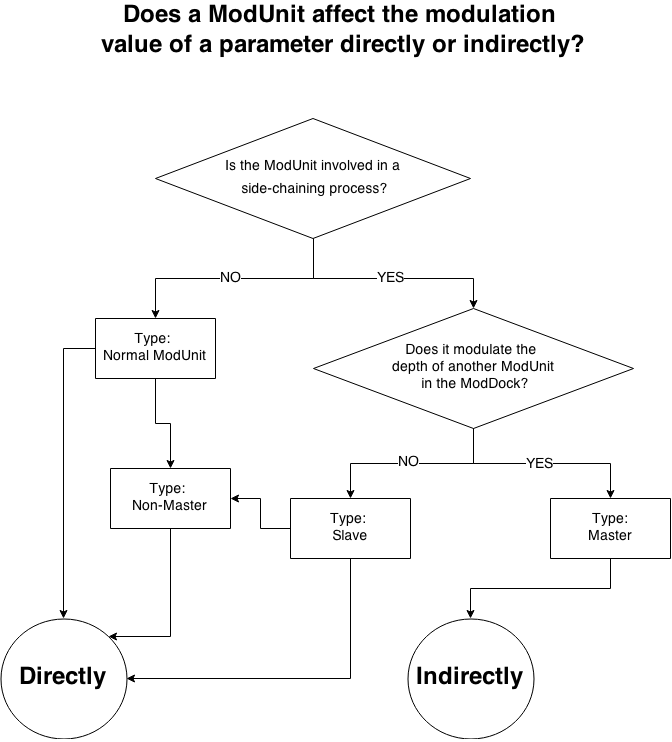
\includegraphics[scale=0.7]{img/flowsc}
  \caption{}
  \label{fig:flowsc}
\end{figure}

\begin{figure}[p!]
  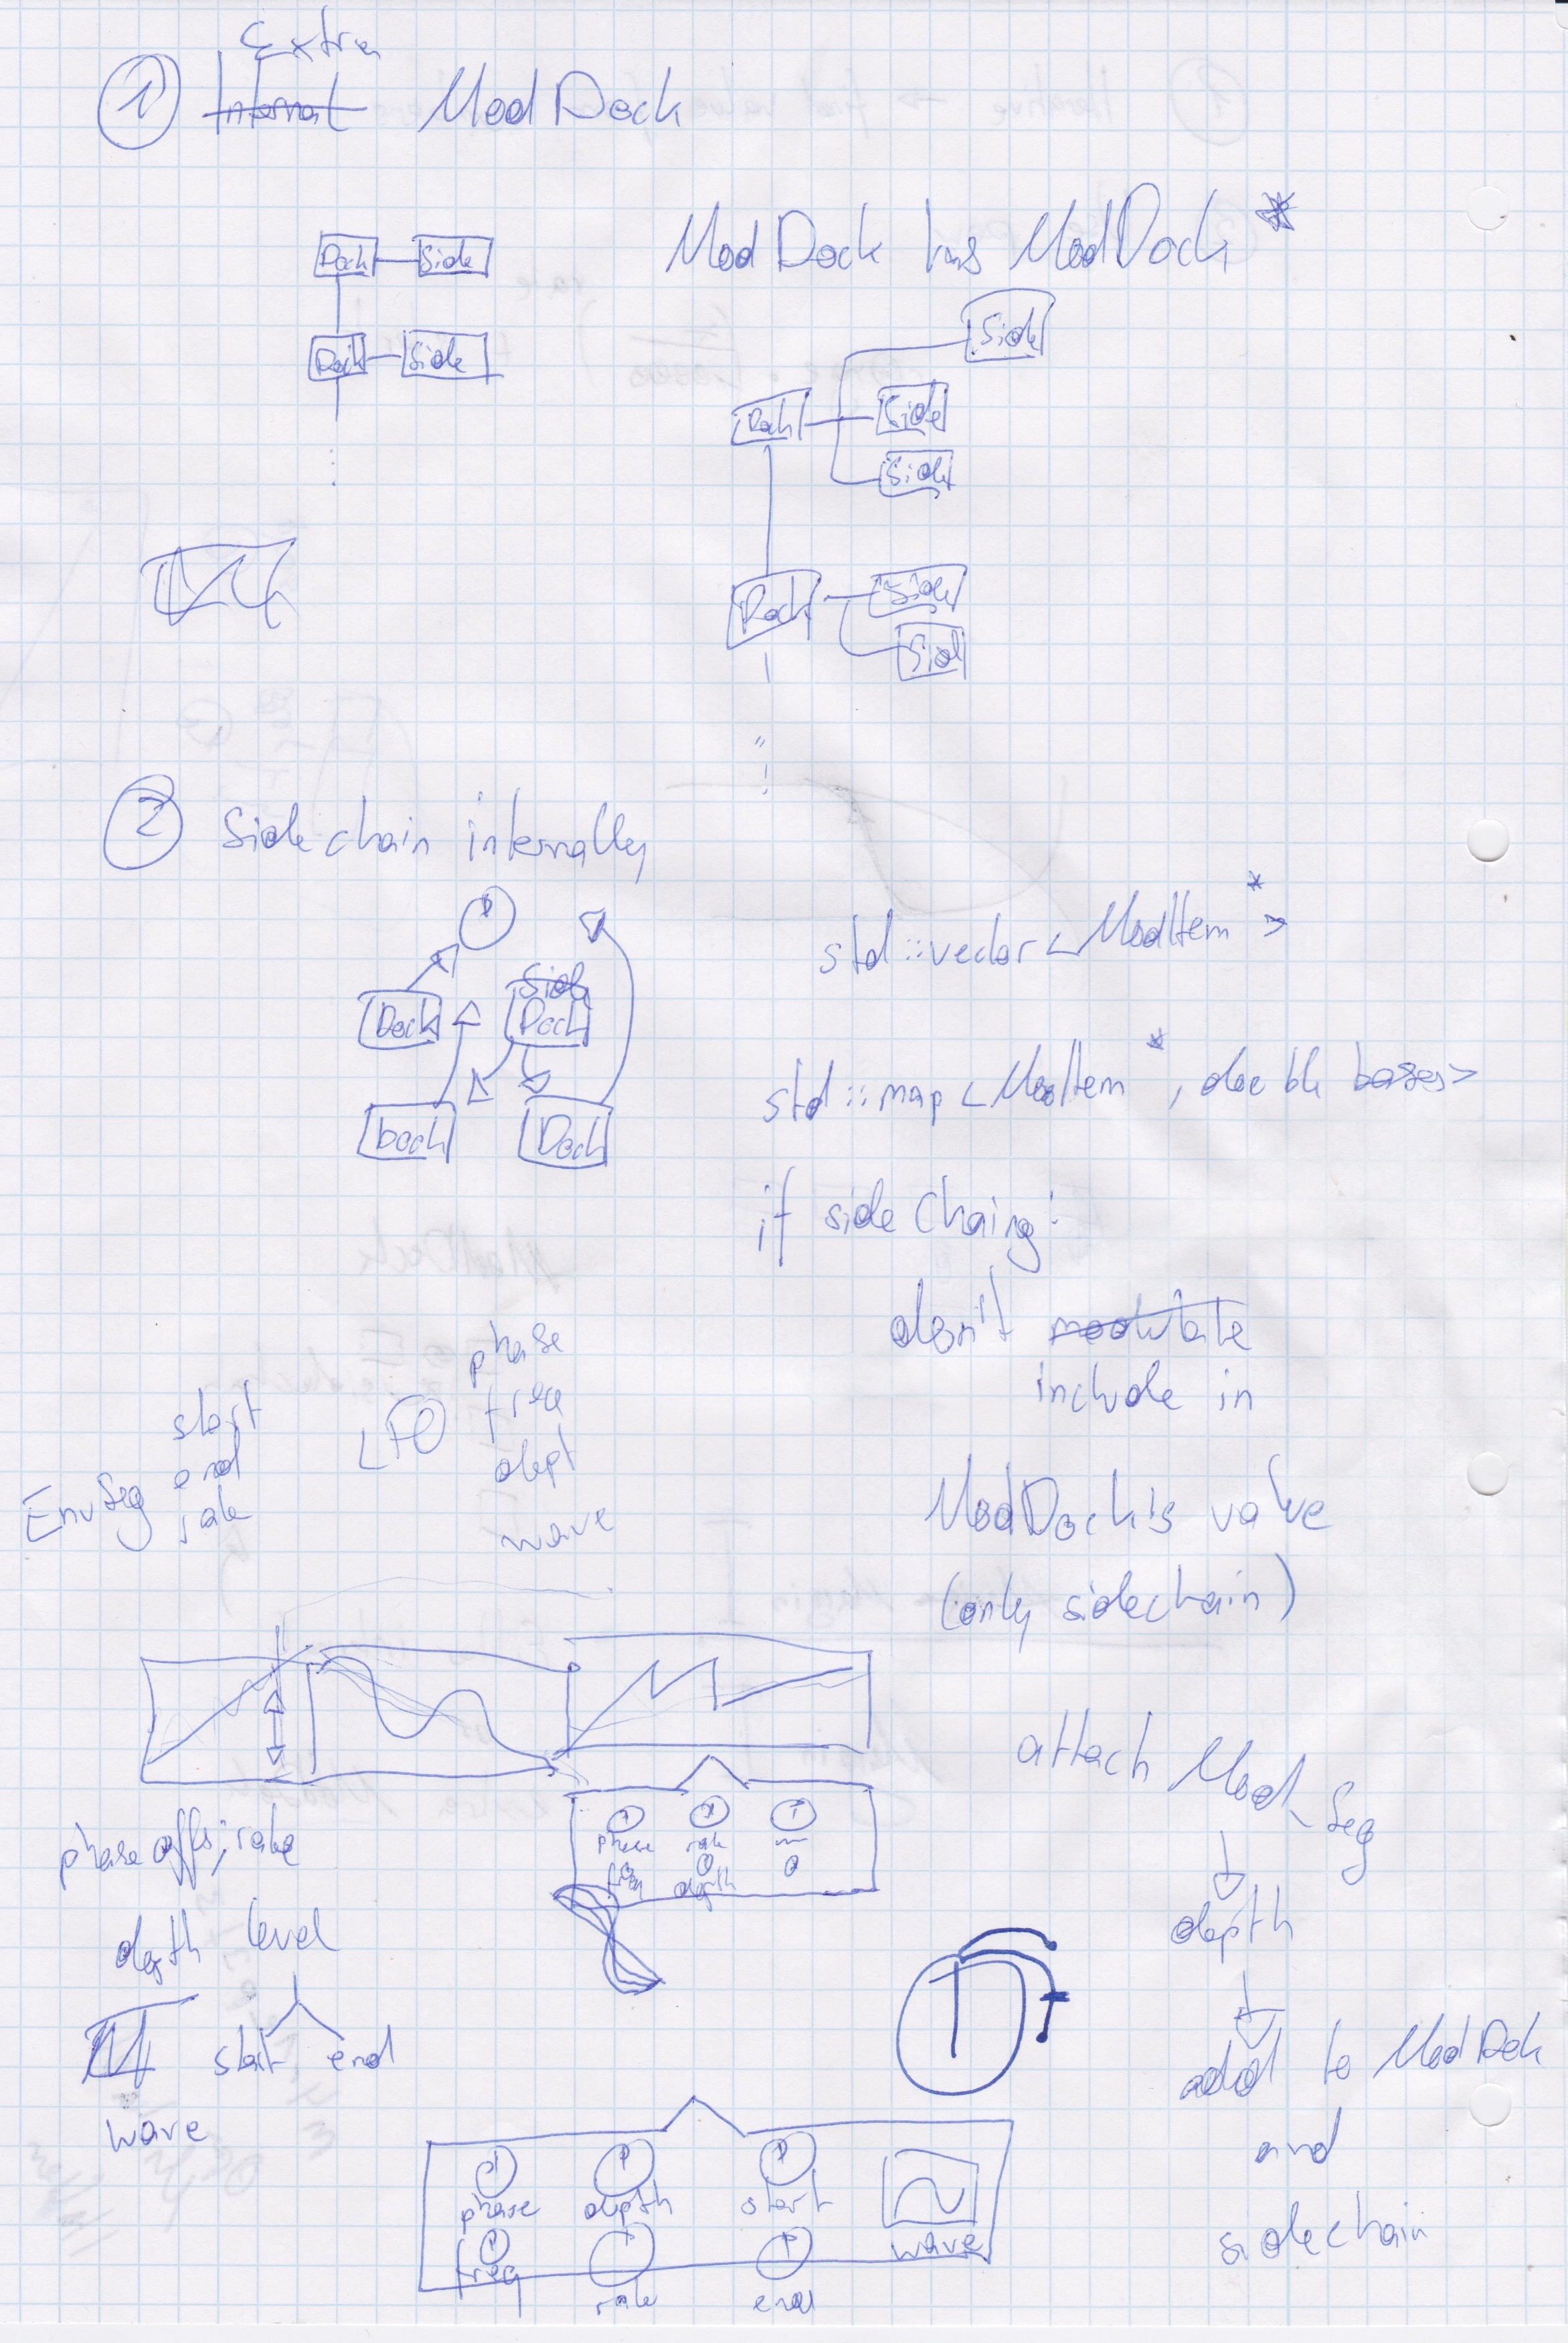
\includegraphics[scale=0.8]{img/scsketch}
  \caption{}
  \label{fig:scsketch}
\end{figure}
